\documentclass[]{beamer}

% Setup appearance:
\mode<presentation>
{
    \usetheme{Berlin}
    \usecolortheme{default}
    \useinnertheme{circles}

    % Define Naturalis colours.
    \definecolor{npink}{HTML}{EE0059}
    \definecolor{nbrown}{HTML}{542E08}
    \definecolor{ngreen}{HTML}{009932}
    \definecolor{ngray}{HTML}{EEEDE9}

    \setbeamercolor{normal text}{fg=black,bg=ngray}
    \setbeamercolor{alerted text}{fg=ngreen}
    \setbeamercolor{example text}{fg=ngreen!50!black}

    \setbeamercolor{structure}{fg=npink} % Main structure highlight colours
    \setbeamercolor{background canvas}{parent=normal text}
    \setbeamercolor{background}{parent=background canvas}

    \setbeamercolor{palette primary}{fg=white,bg=npink} % Title bar
    \setbeamercolor{palette secondary}{use=structure,fg=white} % Section bar
    \setbeamercolor{palette tertiary}{fg=ngray,bg=black} % Navigation bar
}

\usepackage[english]{babel} % apt-get install texlive-lang-english
\usepackage[utf8]{inputenc}
\usepackage[T1]{fontenc}
\usepackage{booktabs} % Pretty rules for tables
\usepackage{enumerate} % Enumerated lists
\usepackage{graphicx} % Loading images
\usepackage{textpos}
\usepackage{wrapfig} % Wrapping text around images
\usepackage{caption} % Advanced features for image/table captions
\usepackage{tikz} % Drawing diagrams
\usetikzlibrary{arrows,backgrounds,fit,shapes}

% Configure caption
\captionsetup{margin=10pt,font=scriptsize,labelfont=bf,labelsep=colon}

% For including images
\DeclareGraphicsExtensions{.pdf,.png,.jpg,.eps}
\graphicspath{{./images/}}

\title[OrchiD]
    {OrchiD: identification of orchid species by means of automated image recognition}

\author[Gravendeel, Pereira, Vos]
    {Barbara Gravendeel\inst{1}, Serrano Pereira\inst{1}, Rutger Vos\inst{1}}

\institute[Naturalis Biodiversity Center]
{
  \inst{1}
  Naturalis Biodiversity Center, The Netherlands
}

%\logo{
\includegraphics[height=1cm]{Naturalis_logo_staand_rood}}

\date{October 23, 2014}

\subject{Bioinformatics}

% Show ToC at beginning of each section
\AtBeginSubsection[]
{
  \begin{frame}<beamer>{Outline}
    \tableofcontents[currentsection,currentsubsection]
  \end{frame}
}

\begin{document}

% Title page
\frame{\titlepage}

% Add logo to title bar
\addtobeamertemplate{frametitle}{}{
    \begin{textblock*}{2cm}(\textwidth, -0.9cm)
        
\includegraphics[height=0.8cm]{Naturalis_logo_small}
    \end{textblock*}
}

% ToC
\begin{frame}
    \frametitle{Outline}
    \tableofcontents
\end{frame}


\section{Introduction}

	% context within which we do this project %
	\subsection{Background}
	\begin{frame}
		\frametitle{Background}
		\begin{itemize}
			\item Natural historians, both private and institutional, have large
			collections of images
			\item Detailed taxonomic expertise is rare and costly
			\item Unassisted feature extraction (e.g. phenotyping) has broad applications
			\item Automated classifiers might sometimes be `good enough'
		\end{itemize}
	\end{frame}

	% explanation of what "unassisted feature extraction" actually is %
	\begin{frame}
		\frametitle{Unassisted feature extraction}
		\begin{itemize}
			\item Assisted feature extraction, e.g. by placing landmarks by hand, is
			labour intensive and cannot scale
			\item Many expert systems automate feature extraction to identify salient
			details in an image. For example:
			\begin{itemize}
				\item Tissues in medical imaging
				\item Pollen grains or forams in drilling cores
				\item Faces of people
			\end{itemize}
		\end{itemize}
	\end{frame}

	% explanation of what "automated classifiers" are %
	\begin{frame}
		\frametitle{Automated classifiers}
		\begin{itemize}
			\item Automated classification of data using machine learning becomes more and
			more important. For example:
			\begin{itemize}
				\item Spam filters
				\item Automated stock trading
				\item Character recognition
			\end{itemize}
			\item Artificial Neural Networks (ANNs) are one commonly-used approach
		\end{itemize}
	\end{frame}

	% more information about ANNs %
    \begin{frame}
        \frametitle{Artificial Neural Networks}

        % Space between neuron layers.
        \def\layersep{2.5cm}
        % Number of input neurons.
        \def\inputneurons{4}
        % Number of hidden neurons.
        \def\hiddenneurons{5}
        % Number of output neurons.
        \def\outputneurons{3}

        % Source: http://www.texample.net/tikz/examples/neural-network/
        \begin{tikzpicture}[shorten >=1pt,->,draw=black!50, node distance=\layersep]
            \tikzstyle{every pin edge}=[<-,shorten <=1pt]
            \tikzstyle{neuron}=[circle,fill=black!25,minimum size=17pt,inner sep=0pt]
            \tikzstyle{input neuron}=[neuron, draw=green!75, fill=green!20];
            \tikzstyle{hidden neuron}=[neuron, draw=blue!75, fill=blue!20];
            \tikzstyle{output neuron}=[neuron, draw=red!75, fill=red!20];
            \tikzstyle{annot} = [text width=4em, text centered]

            % Draw the input layer nodes
            \foreach \name / \y in {1,...,\inputneurons}
            % This is the same as writing \foreach \name / \y in {1/1,2/2,3/3,4/4}
                \node[input neuron, pin=left:Input \y] (I-\name) at (0,-\y) {};

            % Draw the hidden layer nodes
            \foreach \name / \y in {1,...,\hiddenneurons}
                \path[yshift=0.5cm]
                    node [hidden neuron]
                    (H-\name) at (\layersep,-\y cm) {};

            % Draw the output layer node
            \foreach \name / \y in {1,...,\outputneurons}
                \path[yshift=-0.5cm]
                    node [output neuron,
                          pin={[pin edge={->}]right:Output \y},
                          right of=H-\y]
                        (O-\name) at (\layersep,-\y cm) {};

            % Connect every node in the input layer with every node in the
            % hidden layer.
            \foreach \source in {1,...,\inputneurons}
                \foreach \dest in {1,...,\hiddenneurons}
                    \path (I-\source) edge (H-\dest);

            % Connect every node in the hidden layer with the output layer
            \foreach \source in {1,...,\hiddenneurons}
                \foreach \dest in {1,...,\outputneurons}
                    \path (H-\source) edge (O-\dest);

            % Annotate the layers
            \node[annot,above of=H-1, node distance=1cm] (hl) {Hidden layer};
            \node[annot,left of=hl] {Input layer};
            \node[annot,right of=hl] {Output layer};
        \end{tikzpicture}
    \end{frame}

	% outline of our goals %
    \subsection{Goals}
    \begin{frame}
        \frametitle{Goals}
		\begin{itemize}
			\item Simple strategies for managing reference image sets
			\item Automated segmentation and normalization of digital images
			\item Unassisted feature extraction algorithms
			\item ANN `decision trees' that mirror taxonomy
			\item A user-friendly, proof-of-concept web application
        \end{itemize}
    \end{frame}

	% description of the "study system", i.e. slipper orchids %
	\subsection{Study system}
    \begin{frame}
        \frametitle{The Slipper Orchids (Cypripedioideae)}
        \begin{itemize}
            \item Horticulturally popular group
            \item Highly endangered in the wild
            \item Well identifiable based on shape and flower colour
        \end{itemize}

        % Three horizontally aligned images.
        \begin{figure}[!htb]
            \minipage{0.26\textwidth}
              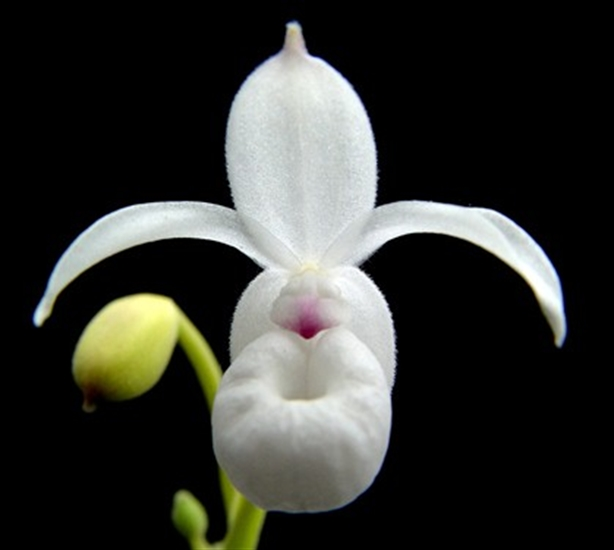
\includegraphics[width=\linewidth]{Mexipedium_xerophyticum}
              \caption*{\textit{Mexipedium xerophyticum}}
            \endminipage\hfill
            \minipage{0.30\textwidth}
              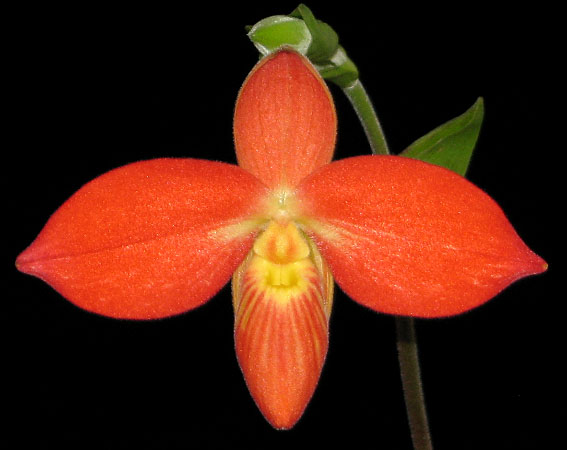
\includegraphics[width=\linewidth]{Phragmipedium_besseae}
              \caption*{\textit{Phragmipedium besseae}}
            \endminipage\hfill
            \minipage{0.28\textwidth}
              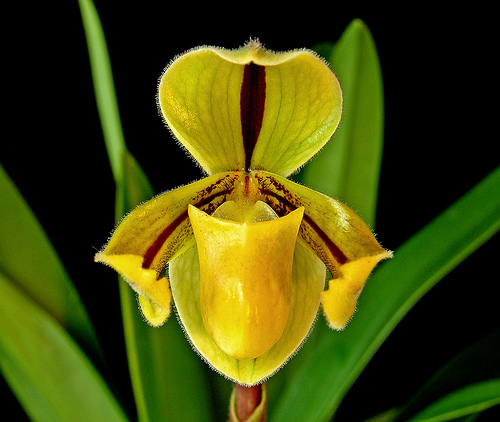
\includegraphics[width=\linewidth]{Paphiopedilum_druryi}
              \caption*{\textit{Paphiopedilum druryi}}
            \endminipage\hfill
        \end{figure}
    \end{frame}


\section{Methods}

	% intro slide about how we manage the images %
    \subsection{Image Management}
    \begin{frame}
        \frametitle{Image Management}

        \begin{minipage}[c]{\textwidth}
            \begin{columns}[T]
                \begin{column}{0.6\textwidth}
                    \begin{itemize}
                        \item Images are collaboratively organized (tagged, copyrights tracked) on
                        a Flickr account
                        \item Image sets are automatically harvested and mirrored locally
                        \item Additional meta data, extracted features and images are stored locally
                    \end{itemize}
                \end{column}
                \begin{column}{0.3\textwidth}
                    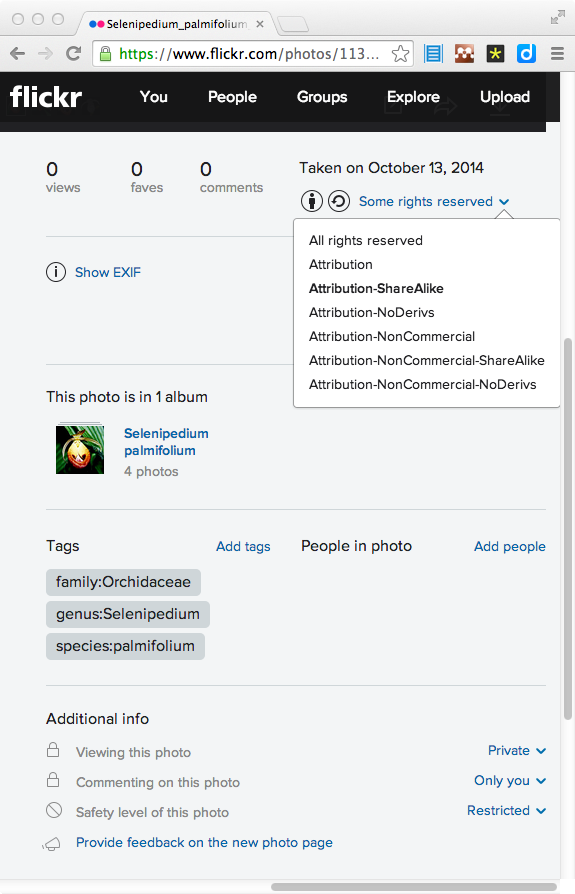
\includegraphics[width=3.5cm]{flickr_metadata}
                \end{column}
            \end{columns}
        \end{minipage}

    \end{frame}

	% database schema %
    \begin{frame}
        \frametitle{Photo Metadata DB}
        \begin{figure}[h]
        \centering
        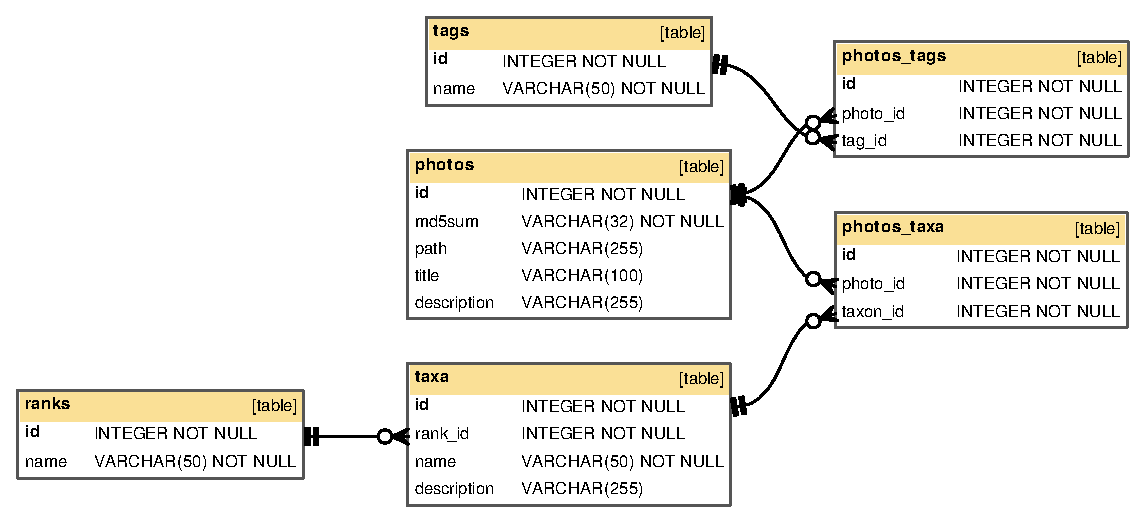
\includegraphics[width=\textwidth]{meta-db-diagram}
        \end{figure}
    \end{frame}


    % image processing (multiple slides) %
    \subsection{Image Processing}

    \begin{frame}[plain]
        \frametitle{Photo Classification Workflow}
        \begin{center}
        \begin{tikzpicture}[node distance=3cm,
                            thick,
                            rounded corners=2pt,
                            auto]
            \tikzstyle{box}=[rectangle,
                            minimum size=6mm,
                            draw=black!50 ,
                            top color=white ,
                            bottom color=black!20]
            \tikzstyle{img}=[inner sep=0pt]

            \node[box] (client)                                {Client};
            \node[box] (prep)           [right of=client,
                                        xshift=3cm]            {Preprocessing};
            \node[box] (feature_ext)    [below of=prep,
                                        yshift=1cm]            {Feature Extraction};
            \node[box] (ann)            [below of=feature_ext,
                                        yshift=0.5cm]          {Neural Networks};

            \draw[->] (client) -- (prep)
                node[midway] {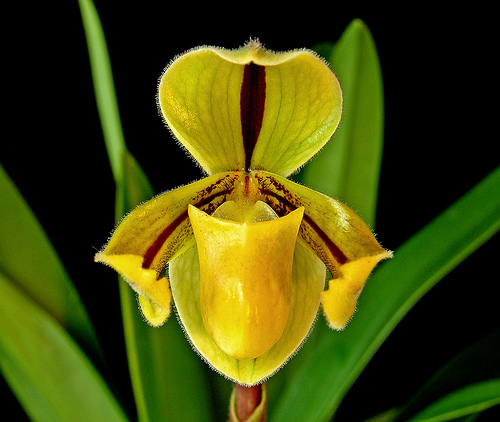
\includegraphics[width=.10\textwidth]{Paphiopedilum_druryi}};
            \draw[->] (prep) -- (feature_ext);
            \draw[->] (feature_ext) -- (ann)
                node[midway] (pheno) {Phenotype};
            \draw[->] (ann.west) -- (client)
                node[midway] (class) {Classification};

            % Background for the server.
            \begin{scope} [on background layer]
                \node [fill=black!20,
                       fit=(prep) (feature_ext) (pheno) (ann),
                       label=above:Server] {};
            \end{scope}
        \end{tikzpicture}
        \end{center}
    \end{frame}

    \begin{frame}[plain]
        \frametitle{Image Processing Workflow}
        \begin{center}
        \begin{tikzpicture}[node distance=3cm,
                            thick,
                            rounded corners=2pt,
                            auto]
            \tikzstyle{box}=[rectangle,
                            minimum size=6mm,
                            draw=black!50 ,
                            top color=white ,
                            bottom color=black!20]
            \tikzstyle{img}=[inner sep=0pt]

            \node[img] (image) {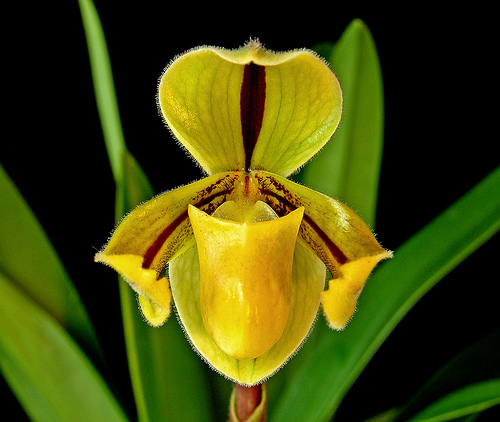
\includegraphics[width=.10\textwidth]{Paphiopedilum_druryi}};
            \node[box] (color correction)   [right of=image]                {Colour Correction};
            \node[box] (segmentation)       [below of=color correction]     {Segmentation};
            \node[box] (feature extr)       [right of=color correction,
                                            xshift=1cm]                     {Colour \& Shape};
            \node[box] (phenotype)          [below of=feature extr]         {Phenotype};

            \draw[->] (image) -- (color correction);
            \draw[->] (color correction) -- (segmentation);
            \draw[->] (segmentation) -- (feature extr);
            \draw[->] (feature extr) -- (phenotype);

            % Background for preprocessing.
            \begin{scope} [on background layer]
                \node [fill=black!20,
                       fit=(color correction) (segmentation),
                       label=above:Preprocessing] {};
            \end{scope}

            % Background for feature extraction.
            \begin{scope} [on background layer]
                \node [fill=black!20,
                       fit=(feature extr) (phenotype),
                       label=above:Feature Extraction] {};
            \end{scope}
        \end{tikzpicture}
        \end{center}
    \end{frame}

    \begin{frame}
        \frametitle{Image Preprocessing}
        \begin{enumerate}
            \item Color correction
                \begin{itemize}
                    \item \textbf{Naik \& Murthy}, 2003. Hue-preserving color image
                    enhancement without gamut problem. \textit{IEEE Transactions on
                    Image Processing} \textbf{12}(12): 1591-1598
                \end{itemize}
            \item Foreground segmentation
                \begin{itemize}
                    \item \textbf{Rother, Kolmogorov \& Blake}, 2004. GrabCut: Interactive
                    Foreground Extraction using Iterated Graph Cuts.
                    \textit{ACM Trans. Graph.} \textbf{23}(3): 309-314
                \end{itemize}
        \end{enumerate}
    \end{frame}

    \begin{frame}[plain]
        \frametitle{Segmentation via GrabCut}
        \begin{center}
        \begin{tikzpicture}
          \node (img1) {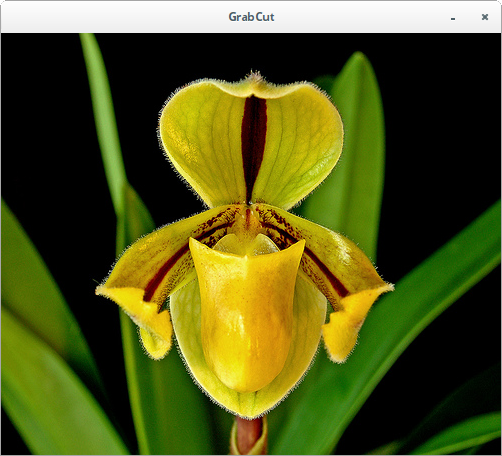
\includegraphics[height=5cm]{GrabCut_druryi_1}};
          \pause
          \node (img2) {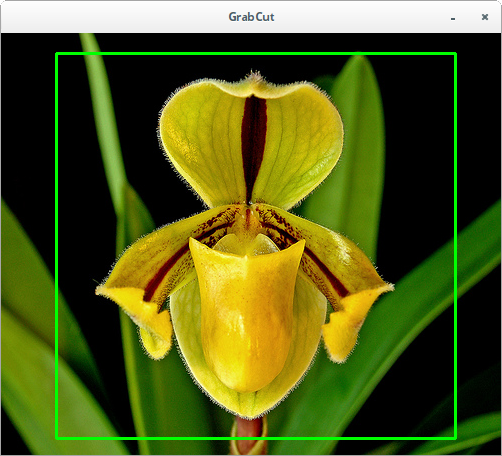
\includegraphics[height=5cm]{GrabCut_druryi_2}};
          \pause
          \node (img3) {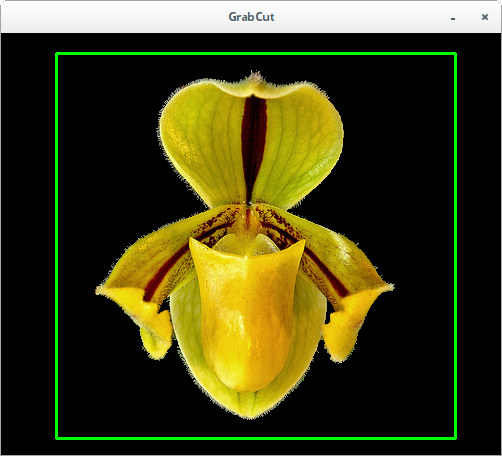
\includegraphics[height=5cm]{GrabCut_druryi_3}};
        \end{tikzpicture}
        \end{center}
    \end{frame}

    \begin{frame}[plain]
        \frametitle{Segmentation via GrabCut}
        \begin{center}
        \begin{tikzpicture}
          \node (img1) {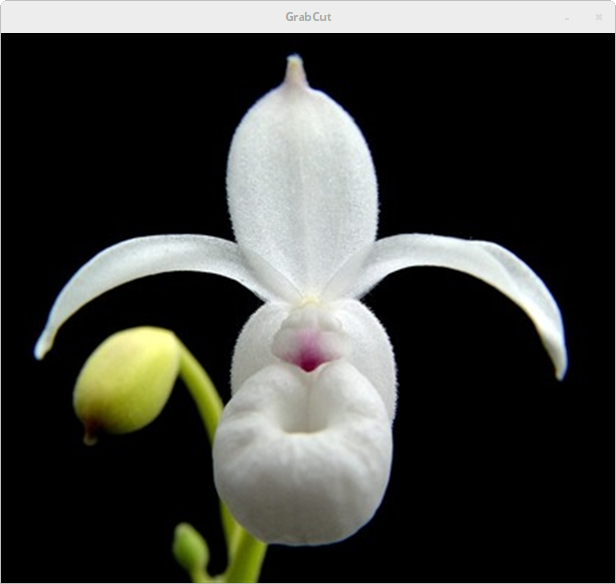
\includegraphics[height=5cm]{GrabCut_xerophyticum_1}};
          \pause
          \node (img2) {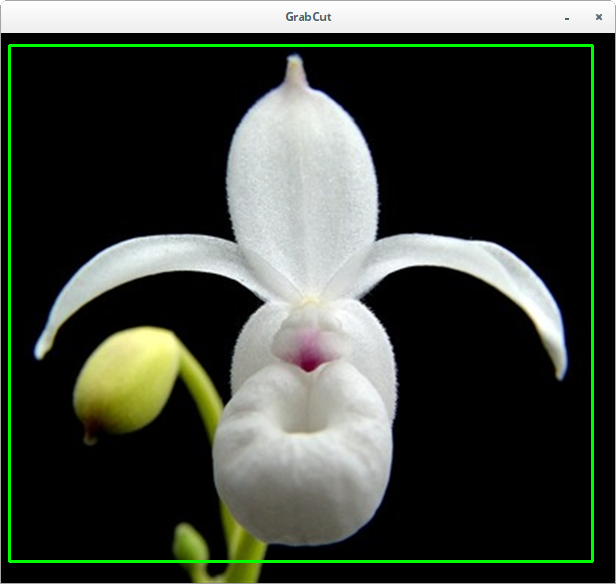
\includegraphics[height=5cm]{GrabCut_xerophyticum_2}};
          \pause
          \node (img3) {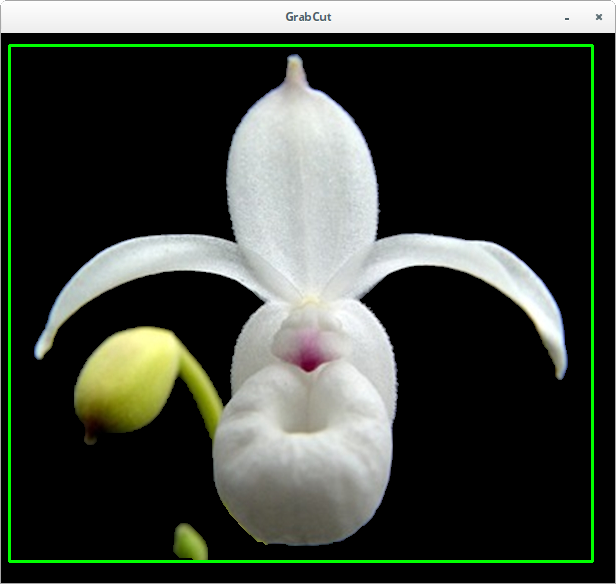
\includegraphics[height=5cm]{GrabCut_xerophyticum_3}};
        \end{tikzpicture}
        \end{center}
    \end{frame}

    \begin{frame}
        \frametitle{Feature Extraction}

        Features (colour \& shape) are extracted from the segmented images.

        \vspace{10 mm}

        \begin{figure}[!htb]
            \minipage{0.28\textwidth}
              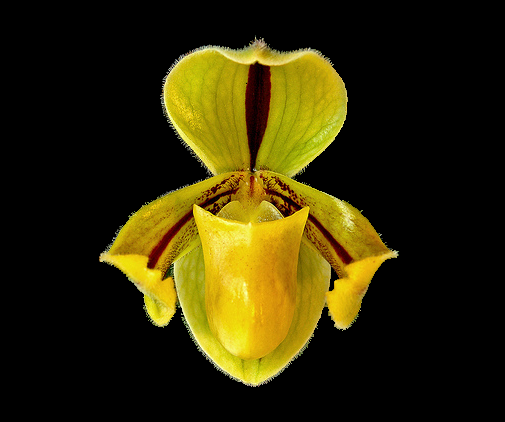
\includegraphics[width=\linewidth]{grabcut_output}
            \endminipage\hfill
        \end{figure}
    \end{frame}

    \begin{frame}[plain]
        \frametitle{Colour and Shape Extraction}
        \begin{figure}[h]
        \centering
        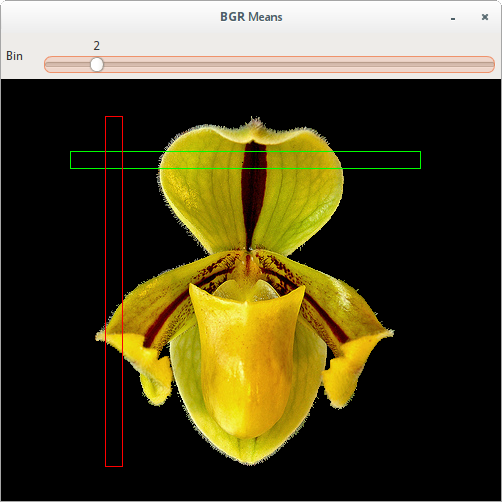
\includegraphics[width=.60\textwidth]{BGR_means_bins}
        \end{figure}
    \end{frame}

    \begin{frame}[plain]
        \frametitle{Colour and Shape Extraction}

        % Two horizontally aligned images.
        \begin{figure}[!htb]
            \minipage{0.50\textwidth}
              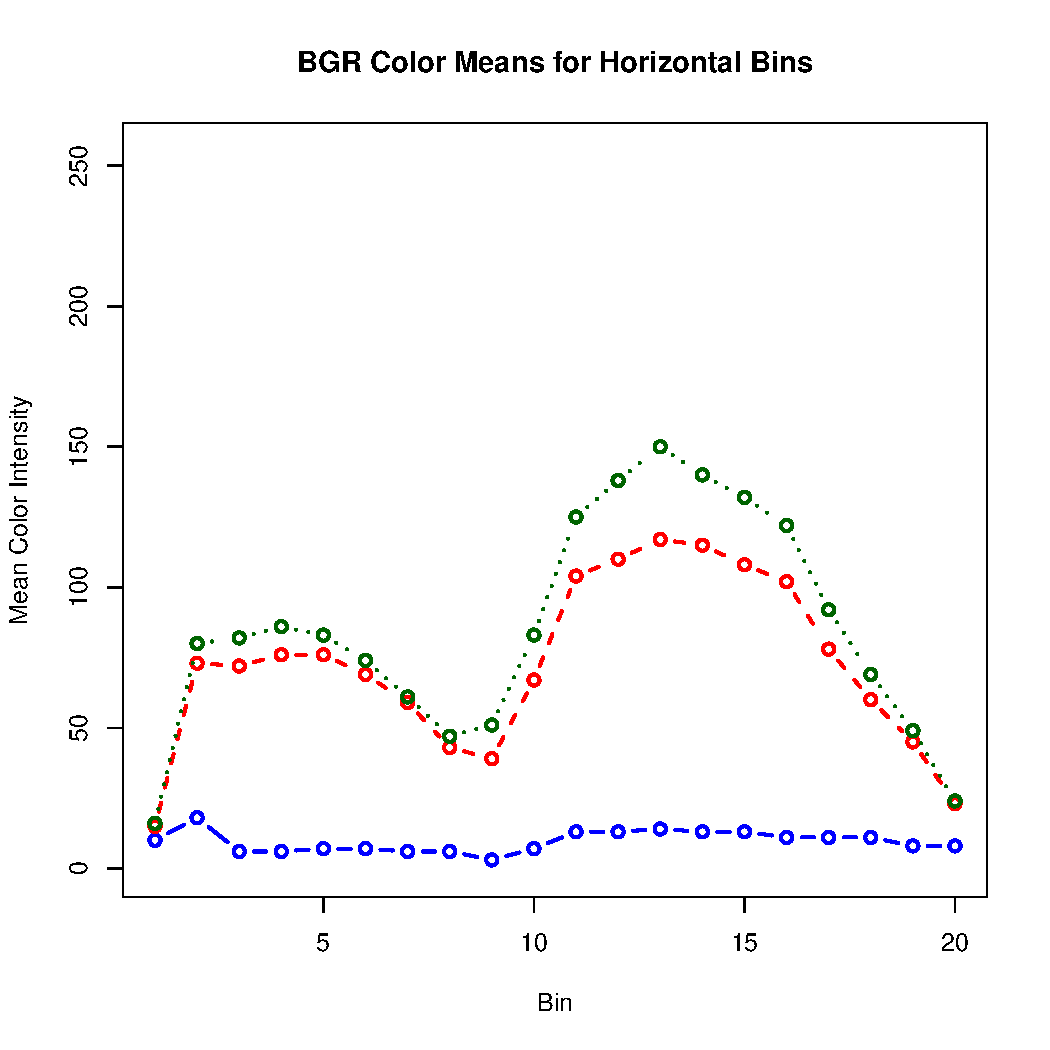
\includegraphics[width=\linewidth]{BGR_means_hor_plot}
            \endminipage\hfill
            \minipage{0.50\textwidth}
              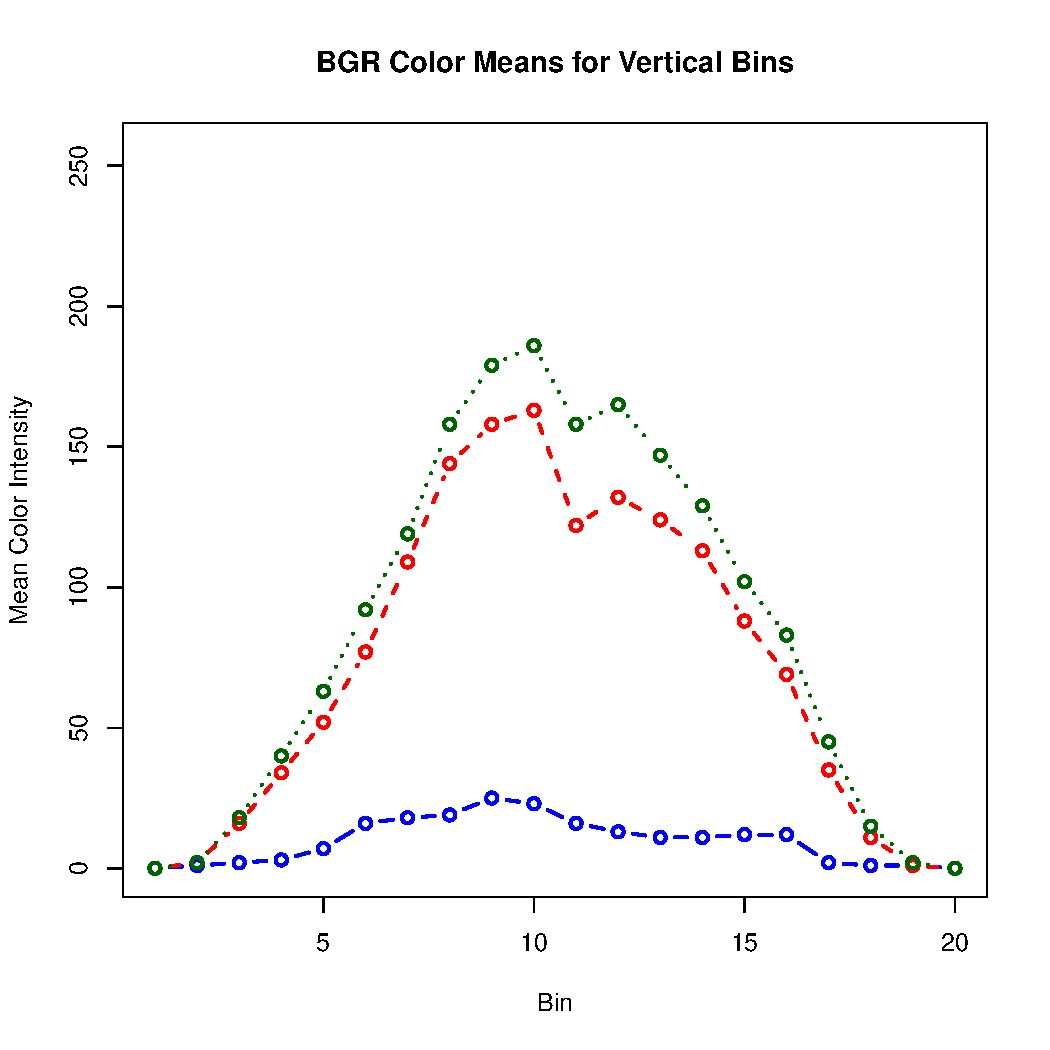
\includegraphics[width=\linewidth]{BGR_means_ver_plot}
            \endminipage\hfill
        \end{figure}
    \end{frame}

    \subsection{Neural Network Training}

    \begin{frame}
        \frametitle{Training Data}

        Format of the training data.

        \begin{table}[h]\scriptsize
            \begin{center}
            \begin{tabular}{lllllll}
            \toprule
            ID & 1.HOR.B & 1.HOR.G & 1.HOR.R & 1.VER.B & 1.VER.G & 1.VER.R \\
            \midrule
            15521194721 & -1 & -1 & -1 & -0.858 & -0.858 & -0.858 \\
            15501195436 & -1 & -1 & -1 & -0.921 & -0.913 & -0.913 \\
            14325862838 & -0.984 & -0.984 & -0.984 & -0.952 & -0.952 & -0.960 \\
            \bottomrule
            \end{tabular}
            \end{center}
        \end{table}
    \end{frame}

    \begin{frame}
        \frametitle{Training Data}

        Codewords used for training.

        \begin{table}[h]\scriptsize
            \begin{center}
            \begin{tabular}{ll}
            \toprule
            \textbf{Class} & \textbf{Codeword} \\
            \midrule
            \textit{Cypripedium}    & \texttt{1 0 0 0 0} \\
            \textit{Mexipedium}     & \texttt{0 1 0 0 0} \\
            \textit{Paphiopedilum}  & \texttt{0 0 1 0 0} \\
            \textit{Phragmipedium}  & \texttt{0 0 0 1 0} \\
            \textit{Selenipedium}   & \texttt{0 0 0 0 1} \\
            \bottomrule
            \end{tabular}
            \end{center}
        \end{table}
    \end{frame}

    \begin{frame}
        \frametitle{Training and Classification}

        \begin{itemize}
            \item ANN `decision trees' that mirror taxonomy{\newline}

            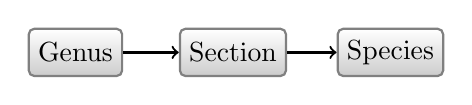
\begin{tikzpicture}[node distance=2cm,
                                thick,
                                rounded corners=2pt]
                \tikzstyle{box}=[rectangle,
                                minimum size=6mm,
                                draw=black!50 ,
                                top color=white ,
                                bottom color=black!20]

                \node[box] (genus) {Genus};
                \node[box] (section) [right of=genus] {Section};
                \node[box] (species) [right of=section] {Species};

                \draw[->] (genus) -- (section);
                \draw[->] (section) -- (species);
            \end{tikzpicture}

            \vspace{5 mm}

        \item Training methods:
            \begin{itemize}
                \item Standard training
                \item Training via genetic algorithm
            \end{itemize}
        \end{itemize}
    \end{frame}


\section{Results}

    \subsection{Results}

    \begin{frame}
        \frametitle{Results}

        \begin{itemize}
            \item A vetted digital image collection
            \item A library of generic image feature extraction algorithms
            \item Trained artificial neural networks
            \item Training and classification methods
            \item A proof-of-concept web application
        \end{itemize}
    \end{frame}

    \begin{frame}[plain]
        \frametitle{Image Collection}

        In total 1127 photos were collected.

        \begin{table}[h]\scriptsize
            \begin{center}
            \begin{tabular}{llll}
            \toprule
            \textbf{Genus} & \textbf{Section Count} & \textbf{Species Count} & \textbf{Photo Count} \\
            \midrule
            \textit{Cypripedium} & 11 & 23 & 141 \\
            \textit{Mexipedium} & 0 & 1 & 4 \\
            \textit{Paphiopedilum} & 7 & 71 & 889 \\
            \textit{Phragmipedium} & 4 & 19 & 89 \\
            \textit{Selenipedium} & 0 & 1 & 4 \\
            \bottomrule
            \end{tabular}
            \end{center}
        \end{table}
    \end{frame}

    \begin{frame}[plain]
        \frametitle{Image Collection}

        A subset of the photo collection with 84 selected photos.

        \begin{table}[h]\scriptsize
            \begin{center}
            \begin{tabular}{llll}
            \toprule
            \textbf{Genus} & \textbf{Section Count} & \textbf{Species Count} & \textbf{Photo Count} \\
            \midrule
            \textit{Cypripedium} & 3 & 4 & 25 \\
            \textit{Mexipedium} & 0 & 1 & 4 \\
            \textit{Paphiopedilum} & 3 & 4 & 31 \\
            \textit{Phragmipedium} & 1 & 3 & 20 \\
            \textit{Selenipedium} & 0 & 1 & 4 \\
            \bottomrule
            \end{tabular}
            \end{center}
        \end{table}
    \end{frame}

    \subsection{Cross Validation}

    \begin{frame}
        \frametitle{K-fold Cross Validation}

        Results for stratified k-fold cross validations.

        \begin{table}[h]\scriptsize
            \begin{center}
            \begin{tabular}{lp{3cm}p{3cm}}
            \toprule
            \textbf{Classification Precision} & \textbf{Accuracy{\newline}k=4} & \textbf{Accuracy (subset){\newline}k=4} \\
            \midrule
            genus                   & 75\% ({$\sigma$} 3 pp)    & 80\% ({$\sigma$} 9 pp) \\
            genus/section           & 46\% ({$\sigma$} 7 pp)    & 61\% ({$\sigma$} 10 pp) \\
            genus/section/species   & 19\% ({$\sigma$} 5 pp)    & 46\% ({$\sigma$} 11 pp) \\
            \bottomrule
            \end{tabular}
            \end{center}
        \end{table}
    \end{frame}

    \subsection{Tools}

    \begin{frame}
        \frametitle{Tools}

        \begin{description}[\texttt{NBClassify}]
            \item[\texttt{AIvolver}] Evolve optimal neural networks.
            \item[\texttt{ImgPheno}] Library of generic image feature extraction algorithms.
            \item[\texttt{NBClassify}] Image harvesting, training, and classification tools.
            \item[\texttt{OrchiD}] Proof-of-concept web application.
        \end{description}

    \end{frame}

    \begin{frame}[plain]
        \frametitle{OrchiD}

        \begin{center}
        \begin{tikzpicture}
          \node (img1) {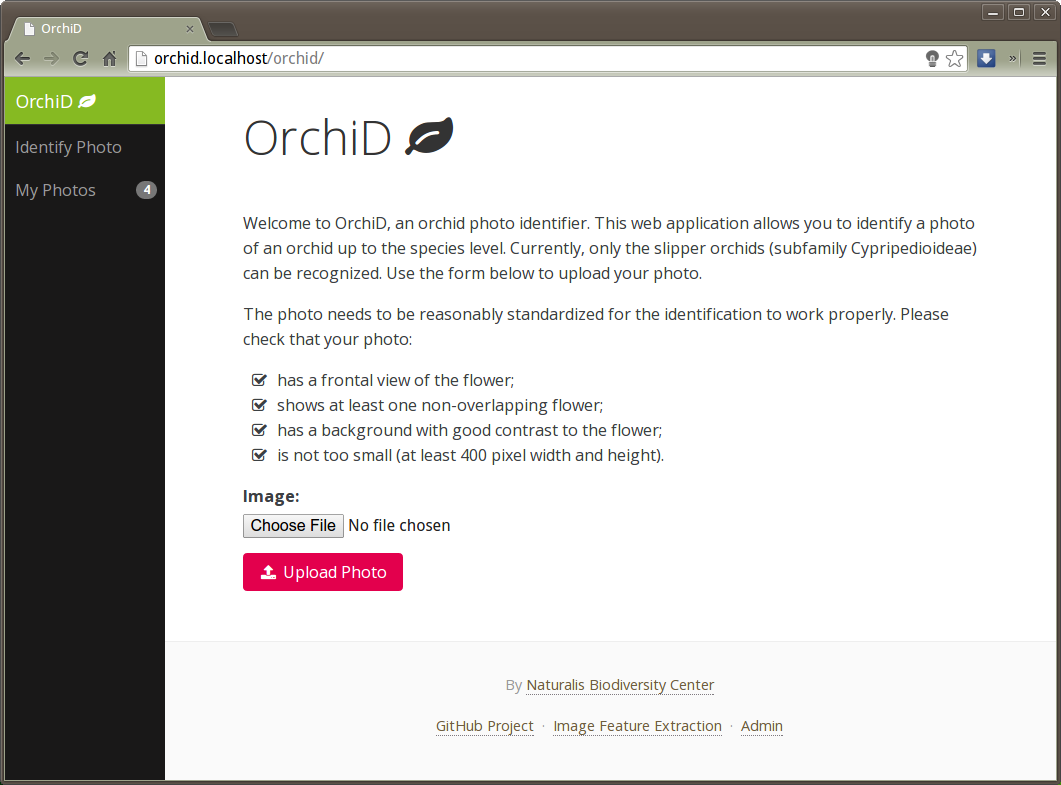
\includegraphics[height=5cm]{OrchiD_1}};
          \node (img2) at (img1.south east) {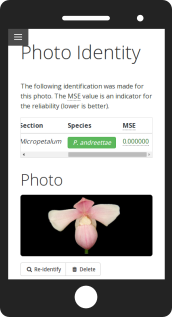
\includegraphics[height=3.5cm]{OrchiD_phone}};
          \pause
          \node (img3) at (img1.south west) {\includegraphics[height=3cm]{Patrick_circle}};
        \end{tikzpicture}
        \end{center}
    \end{frame}

    \begin{frame}[plain]
        \frametitle{OrchiD}

        \begin{center}
        \begin{tikzpicture}
          \node (img1) {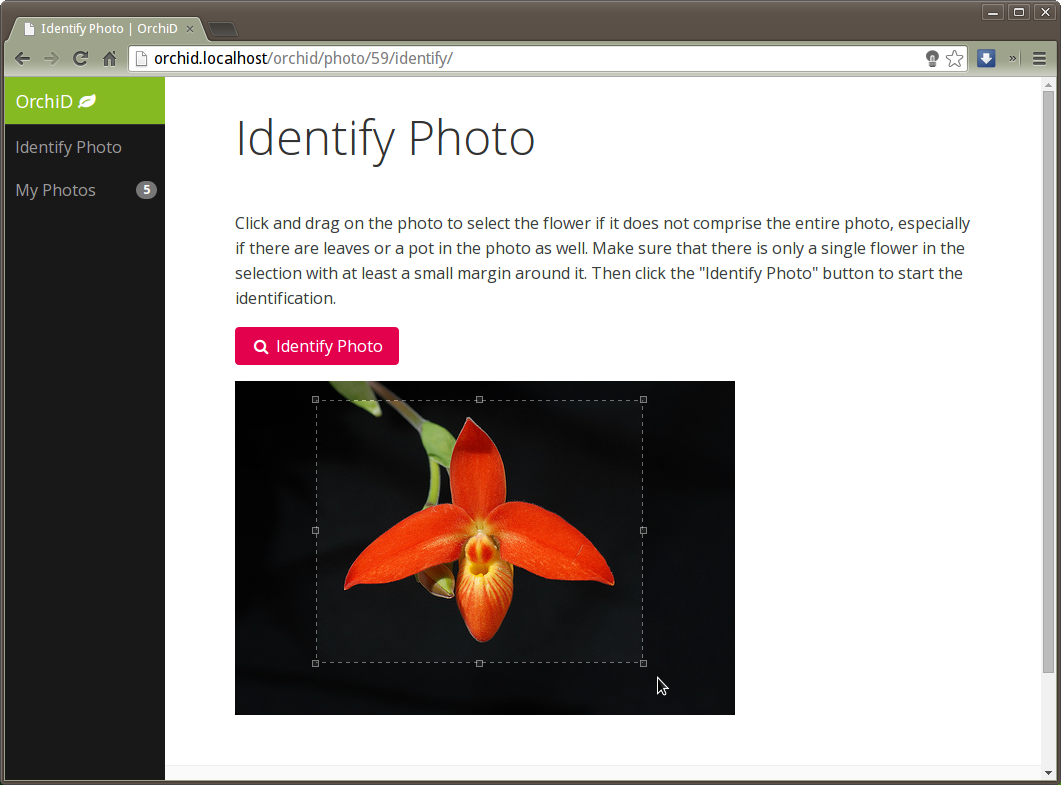
\includegraphics[height=5cm]{OrchiD_2}};
          \pause
          \node (img2) at (img1.south east) {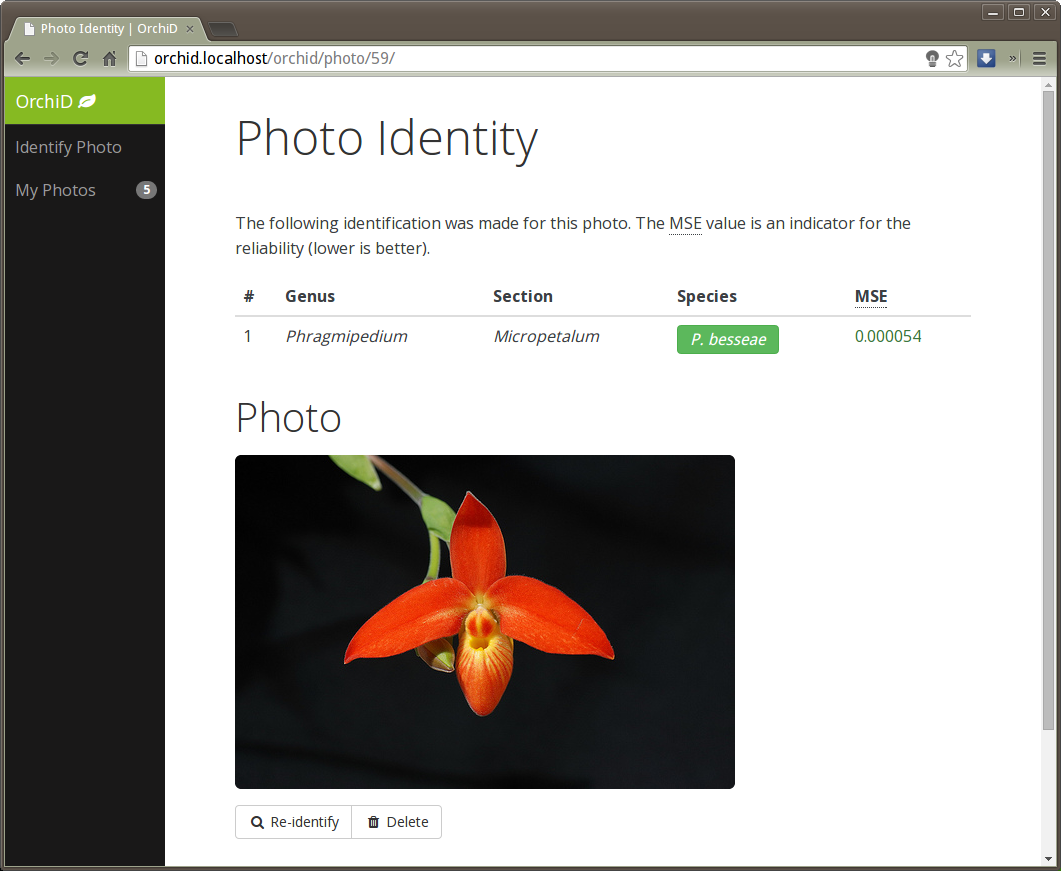
\includegraphics[height=5cm]{OrchiD_3}};
          \pause
          \node (img3) at (img2.south west) [yshift=1cm] {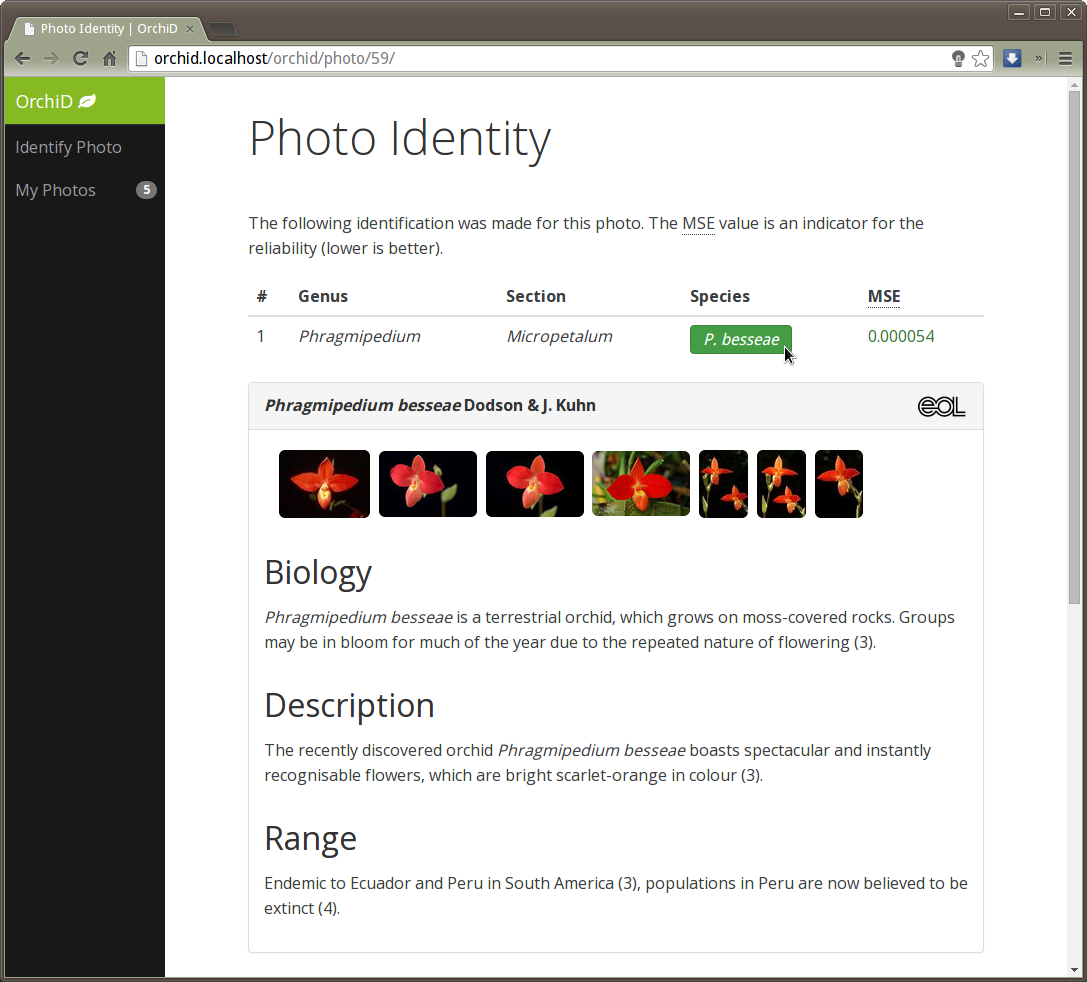
\includegraphics[height=5cm]{OrchiD_4}};
          \pause
          \node (img4) at (img3.north east) [xshift=1cm] {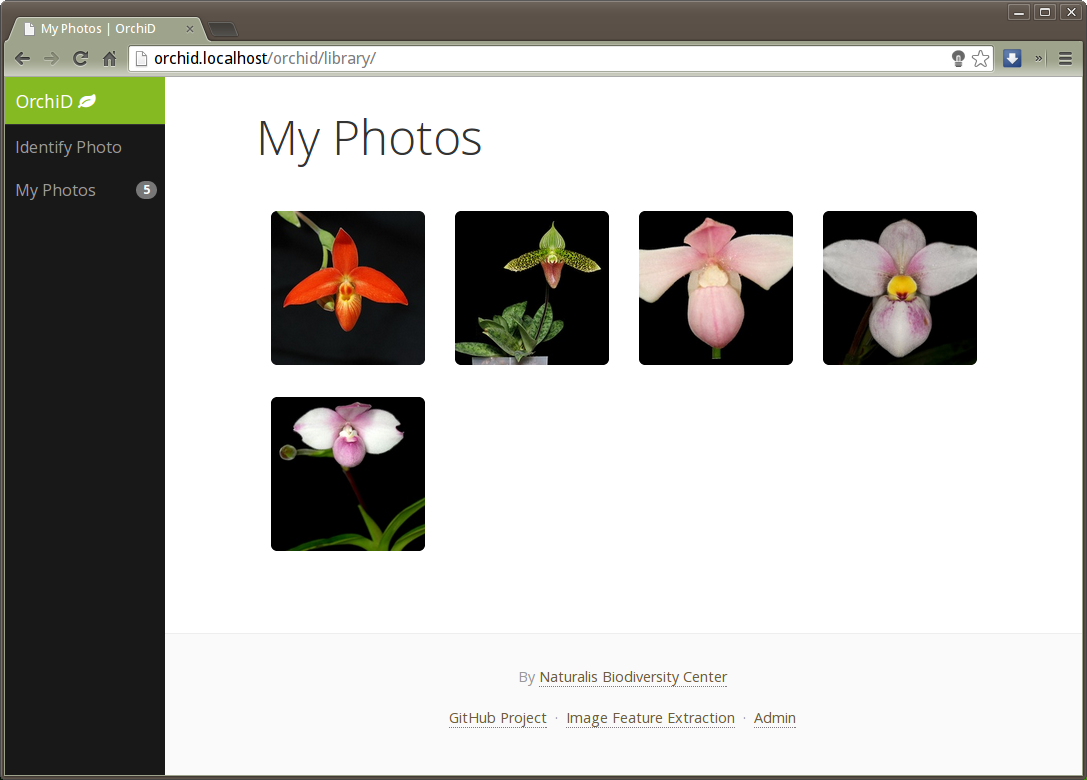
\includegraphics[height=5cm]{OrchiD_5}};
        \end{tikzpicture}
        \end{center}
    \end{frame}

\section{Conclusions}

    \begin{frame}
        \frametitle{Conclusions}

        \begin{itemize}
            \item Classification accuracy needs improvement:
            \begin{itemize}
                \item Training via genetic algorithm
                \item Manually preprocess images for training
                \item Combinations of multiple features
                \item Increase Hamming distances for codewords
                \item Neural network committees
            \end{itemize}
        \end{itemize}

        \begin{itemize}
            \item Outlook
            \begin{itemize}
                \item OrchiD: Mobile App
            \end{itemize}
        \end{itemize}
    \end{frame}


\section*{Acknowledgements}

    \begin{frame}{Acknowledgements}
        \begin{itemize}
            \item Dave Roberts
            \item Hanneke de Wolf
            \item Naturalis Applied Research grant
            \item Nicolas Davin
            \item Patrick Wijntjes
            \item Wouter Addink
            \item 50+ photographers
        \end{itemize}
    \end{frame}

\end{document}
